%-------------------------------------------------------------------------------
\section{Introduction}
%-------------------------------------------------------------------------------

Web applications today own, store, and sell user data, often without the user's knowledge or
explicit consent~\cite{nytimes:fb, npr:data}. This has dangerous consequences for both users and
application developers, as data leaks lead to loss of livelihoods and
lawsuits~\cite{breach:amazon,breach:twitter, breach:fb, breach:marriott, breach:quora}. Granting web
applications complete ownership of personal data clearly fails to protect users' privacy. 

However, the other extreme is equally problematic.  While strong privacy is clearly desirable,
complete user data ownership results in an arguably even less desirable world for users. While
desirable world for users. While possible~\cite{amber, w5, blockstack, bstore}, such a model results
in inefficient and reduced application utility, leading to a lack of adoption in practice.  
\lyt{I moved the more extended explanation of this to after we bring up our subscription model, since I
wanted to more quickly get to our contribution.}

This paper proposes a new paradigm that grants users flexible privacy when using web
applications, balancing users' desire for privacy with their desire for application utility. In this \emph{subscription} paradigm of interaction, users subscribe to applications by granting a time-limited
lease to their data, with the provision that the application may retain only de-identified
information once the user unsubscribes. Users flexibly switch between a privacy-preserving
unsubscribed mode and an identity-revealing subscribed mode at any time without permanently losing
their data. 
A subscription paradigm contrasts with the current state of web application privacy today,
in which applications have complete ownership of personal data, and the other extreme world of
strong privacy, in which the user has complete data ownership (see Figure~\ref{fig:world}). 

A subscription paradigm clearly benefits users: they can choose privacy at any time, without permanently
losing their accounts or affecting the utility of the applications for others.
Just as importantly, a subscription paradigm  also benefits application developers. Recent laws
such as the European Union's General Data Protection Regulation (GDPR)~\cite{eu:gdpr} and
California's Consumer Privacy Act (CCPA)~\cite{ca:privacy-act} codify users' rights to data
ownership, granting users the right to request erasure of information related to them. Supporting
a subscription paradigm enables applications to comply with these legal mandates, while still allowing its departing users
to easily come back: if applications must let users leave, it is in their best interest to make it
easy for them to return.  

Furthermore, applications can continue to operate using their current revenue model, maintaining performance,
reliability, and utility for their users. 
Because applications retain use of subscribed users' data, and de-identified data of unsubscribed
users, applications optimize the amount of data available to generate profit and provide utility for
subscribed users. The application holds only identifying data for currently subscribed
users, reducing the amount of compromising data in the system to only those users who have
actively agreed to temporarily give up their privacy.

\lyt{TODO make stronger---3step argument.}

However, even with legal incentives in place, this subscription paradigm is far from realized.
Unsubscription is often impossible or cumbersome (users often contact the developers or customer
support directly in order to unsubscribe)~\cite{jdm}, and developers manually implement
coarse-grained, error-prone, and often incomplete unsubscription that fails to completely
de-identify the user. Even worse, no existing application (to our knowledge) supports
privacy-preserving unsubscription with the possiblity of resubscription.  Application unsubscription
thus permanently deletes years or even decades of accumulated application data, costing both users
and the web application, and creating little incentive for the application to support easy
unsubscription. 

In order to make flexible data ownership possible, we must solve the many challenges faced by
application developers. Key among these are the requirements to selectively retain unsubscribed
users' data for legal or application purposes while properly de-identifying this data, and to allow
the user to resubscribe at any time to their last-known subscribed state. The complex data
transformations required by user unsubscription and resubscription highlight the need for new tools
that allow developers to easily and systematically automate the process. As a first step, we propose
\sys, a system that provides abstractions and mechanisms to help developers of databased-backed web
applications achieve correct, privacy-compliant user unsubscription and resubscription without
onerous labor, and without adding undue overheads.

\begin{figure*}[ht!]
    \centering
    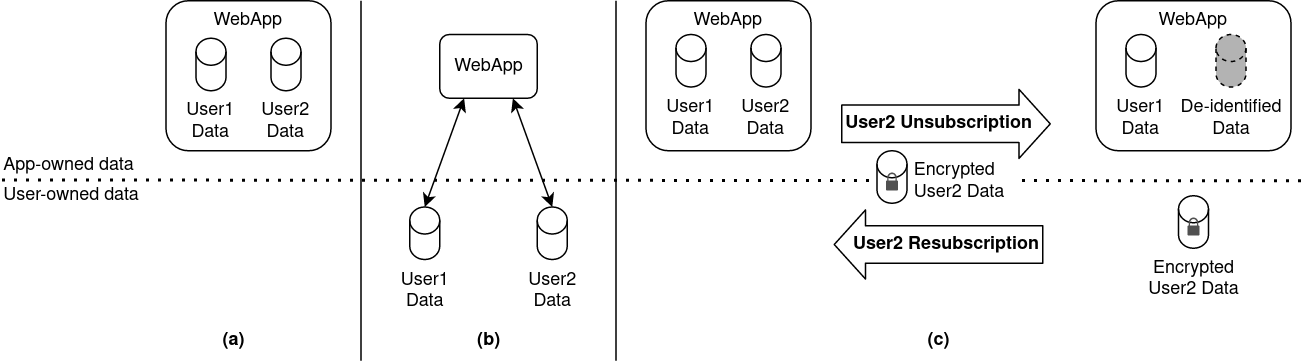
\includegraphics[width=\textwidth]{img/worlds}

    \caption{\textbf{(a)} The existing world of web applications, with applications maintaining and
    owning user data; \textbf{(b)} A world in which users have complete ownership of their data in cloud or local
    storage, and grant applications access to their data;
    \textbf{(c)} Our proposed subscription paradigm, which allows users to switch between privacy-preserving unsubscribed mode (right) and identity-revealing subscribed mode (left).}
    \label{fig:world}
\end{figure*}

\lyt{This paragraph seems more fitting for related work?}
Our proposed subscription paradigm contrasts with the current state of web application privacy today,
in which applications have complete ownership of personal data, and the other extreme world of
strong privacy, in which the user has complete data ownership (see Figure~\ref{fig:world}).  While
strong privacy is clearly desirable, complete user data ownership results in an arguably even less
desirable world for users. While possible~\cite{amber, w5, blockstack, bstore}, applications
must compute on per-user, filesystem-esque storage, \eg as JavaScript in users' browsers in
Blockstack~\cite{blockstack} and BStore~\cite{bstore}. Applications face the loss of the flexibility
and ease of programming over SQL databases with application-specific schemas, and users must decide
on appropriate access control and authentication policies. As a result, service-side computation and
data sharing between users---a large reason users use applications to begin with---becomes
inefficient and impractical. 
%
Furthermore, users are burdened with long-term data maintenance and storage: solutions that use PKI
(\eg Blockstack~\cite{blockstack}) require users to maintain a
master private key, a cumbersome and fragile solution in which losing the key results in permanent
loss of all the user's data.
%
Finally, users must change the way they pay for services, as the current revenue model for
applications relies on access to user data. 
\lyt{this might not be a bad thing, though}.

By supporting a subscription paradigm, applications do not need to access any removed unsubscribed users' data,
simplifying the secure storage of this data when users enter privacy-preserving mode. Applications
can operate as they currently do, with the additional support for users to take back their data and
privacy whenever they wish.
